\documentclass[10pt,twocolumn]{article}

\usepackage[margin=0.72in,columnsep=0.24in]{geometry}
\usepackage[T1]{fontenc}
\usepackage[utf8]{inputenc}
\usepackage{newtxtext,newtxmath}
\usepackage{microtype}
\usepackage{graphicx}
\usepackage{booktabs}
\usepackage{tabularx}
\usepackage{multirow}
\usepackage{array}
\usepackage{enumitem}
\usepackage{xcolor}
\usepackage{hyperref}
\usepackage[round,authoryear]{natbib}
\usepackage{tikz}
\usetikzlibrary{arrows.meta,positioning,fit,calc,shapes.geometric}
\usepackage[font=small,labelfont=bf]{caption}
\usepackage{subcaption}
\usepackage{balance}

\definecolor{navy}{HTML}{17365D}
\definecolor{blue}{HTML}{2F75B5}
\definecolor{lightblue}{HTML}{EAF2F8}
\definecolor{green}{HTML}{548235}
\definecolor{lightgreen}{HTML}{EAF4E3}
\definecolor{orange}{HTML}{C55A11}
\definecolor{lightorange}{HTML}{FCE4D6}
\definecolor{reviewred}{HTML}{9C0006}
\definecolor{reviewfill}{HTML}{FFC7CE}

\hypersetup{
  colorlinks=true,
  linkcolor=navy,
  citecolor=navy,
  urlcolor=blue,
  pdfauthor={Himanshu Jhawar and Sharyn O'Halloran},
  pdftitle={A Human-in-the-Loop Workflow for Reproducible LLM Coding of Legal Delegation and Administrative Discretion}
}

\setlength{\parindent}{1em}
\setlength{\parskip}{0pt}
\setlist{nosep,leftmargin=*}
\renewcommand{\arraystretch}{1.08}
\newcommand{\systemname}{Delegation Workflow Studio}
\newcommand{\future}[1]{\textit{#1}}

\title{\vspace{-1.2em}\textbf{A Human-in-the-Loop Workflow for Reproducible LLM Coding of Legal Delegation and Administrative Discretion}}

% \author{
% Himanshu Jhawar\\
% Columbia University\\
% \texttt{hj2713@columbia.edu}
% \and
% Sharyn O'Halloran\\
% Columbia University\\
% \texttt{so33@columbia.edu}
% }

\date{\small Draft for discussion}

\begin{document}
\maketitle

\begin{abstract}
The growing use of large language models (LLMs) for social-science coding creates a methodological tension: models can accelerate document analysis, but a single prompt obscures how concepts are operationalized, how intermediate judgments affect final labels, and where expert correction enters the process. We present \systemname{}, a research prototype for coding congressional delegation and administrative discretion in U.S. financial-regulation laws. The prototype converts a progressively refined prompt family into an explicit, dependency-aware workflow whose stages, prompts, outputs, conditions, and validation checks are visible and editable. It supports two forms of human intervention: method-level revision of the codebook and workflow, and case-level inspection, correction, or re-evaluation of coded values with retained history. We document the development path from one-shot prompts to staged prompts and then to versioned workflow graphs, using a professor-provided historical coding as the operational ground truth for benchmark alignment. Preliminary binary results illustrate why class-specific evaluation matters: a looser prompt obtains higher raw accuracy on a highly imbalanced benchmark, whereas a stricter prompt substantially improves detection of the rare non-delegation class and balanced accuracy. The contribution is therefore not a claim that an LLM replaces expert coding. It is a design for making expert-guided computational coding inspectable, revisable, and reproducible.
\end{abstract}

\section{Introduction}

Researchers who study political institutions routinely convert complex legal and policy texts into structured variables \citep{grimmer2013text}. In the present project, the substantive task is to identify whether a law delegates meaningful authority to an administrative actor and, conditional on delegation, to characterize the residual discretion available to that actor. Historically, such judgments have been made by trained researchers applying a coding protocol to legislative summaries. The approach is interpretable but costly to scale, especially when the goal is to compare many laws, preserve supporting evidence, and revisit classifications after the codebook changes.

LLMs offer a plausible acceleration mechanism: general annotation studies report substantial cost and performance advantages in some predefined tasks \citep{gilardi2023chatgpt}, and human--LLM frameworks have reduced effort in iterative qualitative coding \citep{dai2023llm}. Prompt-only automation is nevertheless not a sufficient research design for a specialized legal construct. A long prompt may contain definitions, exceptions, stage ordering, and output rules, yet the resulting method remains difficult to audit. When a final rank is wrong, it may be unclear whether the model missed an administrative actor, over-counted a technical amendment, ignored a statutory constraint, or simply failed to follow the required ordering. Prompt changes can also improve one class while degrading another, an important concern when the benchmark distribution is highly imbalanced. Recent evidence on domain-expert legal coding likewise cautions that instruction-prompted generative models can perform poorly on complex constructs even when given the human codebook \citep{thalken2023modeling}.

This paper reports the design and preliminary evaluation of \systemname{}, a human-in-the-loop research prototype that treats the \emph{workflow} rather than an isolated prompt as the unit of the coding method. The workflow exposes ordered stages, dependencies, typed intermediate variables, deterministic branches, and final outputs. Researchers can edit prompts and node settings, test a workflow on a law, inspect a node-level trace, publish a versioned snapshot, and correct selected case-level outputs without silently rewriting the underlying model result.

\medskip
The paper makes four contributions:

\begin{enumerate}
  \item It reconstructs the methodological progression from one-shot classification to staged, dependency-aware coding of delegation and discretion.
  \item It describes a visual workflow representation that makes the operational codebook editable by domain researchers and preserves intermediate evidence for audit.
  \item It defines two explicit human loops: method-level workflow refinement and case-level correction or targeted re-evaluation.
  \item It presents preliminary benchmark evidence showing that raw accuracy can misrepresent progress under severe class imbalance, motivating class-specific recall, balanced accuracy, and law-level disagreement review.
\end{enumerate}

\section{Research Setting}

\subsection{Delegation and discretion}

The project concerns congressional delegation to administrative actors in financial-regulation legislation. The substantive foundation follows a transaction-cost account of delegation \citep{epstein1999delegating} and prior quantitative analysis of U.S. financial-market regulation \citep{groll2021delegation}. The prompt family defines a delegation as a grant of authority to implement, administer, enforce, supervise, regulate, interpret, approve, deny, waive, certify, investigate, or issue rules. The later benchmark-aligned definition is deliberately narrower: a law counts as delegation only when it creates \emph{new} authority or \emph{materially expands} existing authority. Mere agency mentions, reporting duties imposed only on private actors, conforming amendments, and reductions of existing regulation are excluded.

Delegation and discretion are related but distinct concepts. Delegation asks whether an administrative actor receives meaningful authority. Discretion asks how much residual choice remains after statutory goals, procedures, formulas, oversight, deadlines, reporting requirements, review provisions, and other constraints are taken into account. The current ordinal coding uses five ranks:

\begin{description}[style=nextline,leftmargin=0pt,font=\normalfont\bfseries]
  \item[0 --- No delegation.] No qualifying authority is delegated.
  \item[1 --- Narrow or ministerial.] Duties are substantially specified and leave little policy choice.
  \item[2 --- Bounded discretion.] Choice exists but is structured by criteria, formulas, procedures, or oversight.
  \item[3 --- Meaningful policy choice.] The actor can make consequential choices within a recognizable statutory framework.
  \item[4 --- Broad policy-shaping authority.] Authority is durable and wide, with relatively few meaningful constraints.
\end{description}

This formulation follows the language embedded in the professor-provided prompts, capturing the structural distinctions between ministerial duties (Rank 1), bounded decision-making (Rank 2), policy choices (Rank 3), and broad delegation (Rank 4).

\subsection{Benchmark and source discipline}

The operational benchmark is a professor-provided historical coding of \texttt{DelegateLaw} and \texttt{Discretion\_Rank}. We refer to it as the project's \emph{ground truth} for benchmark alignment, while recognizing that it represents a historical social-science coding rather than an adjudication of legal truth.

The source universe is methodologically important. The historical labels were produced from CQ summaries or corresponding descriptions of major provisions. Full statutory text can contain technical or minor delegations absent from those summaries. Consequently, a full-text model may be legally plausible while disagreeing with the historical label for reasons unrelated to prompt quality. Benchmark runs therefore use the same summary-level information set; full-text runs are labeled exploratory.

The repository currently contains 169 summary files (161 delegation-positive and eight delegation-negative) spanning 1950--2013, which represent the intersection of historical legislative records and available summaries. The broader, unlabeled document database in the prototype extends through 2020 (totaling 412 documents), while the ground-truth benchmark CSV contains 121 manually coded financial laws spanning 1950--2013.

\section{Related Work}

\subsection{LLMs as research coders}

LLMs have shown promise as low-cost annotators. \citet{gilardi2023chatgpt} report that ChatGPT outperformed crowd workers on several text-annotation tasks, while \citet{dai2023llm} demonstrate an iterative human--LLM process for thematic analysis. Human-centric work has also emphasized assisting coders rather than treating full automation as the only objective, particularly when rare codes and coder-specific practices matter \citep{spinosodipiano2023qualitative}.

These results do not establish reliability for specialized legal constructs. Legal NLP benchmarks such as LexGLUE and LegalBench emphasize task-specific evaluation and expert-designed categories \citep{chalkidis2022lexglue,guha2023legalbench}. More directly, \citet{thalken2023modeling} find that prompted generative models performed poorly when applying a domain-expert codebook to historical Supreme Court opinions, with their strongest results instead coming from an in-domain fine-tuned model. This contrast motivates our conservative position: LLM coding is evaluated against a controlled benchmark and remains subject to expert review.

\subsection{Expert supervision and workflow authoring}

Weak supervision provides one model for converting expert heuristics into reusable computational signals \citep{ratner2017snorkel}; technology-assisted review in legal discovery likewise demonstrates iterative human feedback over ranked documents \citep{cormack2014evaluation}. Our current prototype does not learn a weak-supervision label model and does not implement a formal active-learning queue. It instead operationalizes the expert codebook directly as a versioned executable workflow.

Visual prompt-chaining systems are important predecessors. AI Chains decomposes LLM tasks into modular, controllable steps \citep{wu2022aichains}, while PromptChainer provides node-edge authoring, per-step testing, intermediate-output inspection, and debugging for chained prompts \citep{wu2022promptchainer}. We therefore do not claim to invent human-in-the-loop annotation or visual prompt chaining. Our contribution is their integration into a research instrument for law-level delegation and ordinal discretion coding, with typed institutional variables, deterministic branches, benchmark mapping, source-policy controls, document-level traces, and separate method- and case-level interventions.

\section{From Prompts to an Explicit Workflow}

\begin{figure*}[t]
\centering
\resizebox{\textwidth}{!}{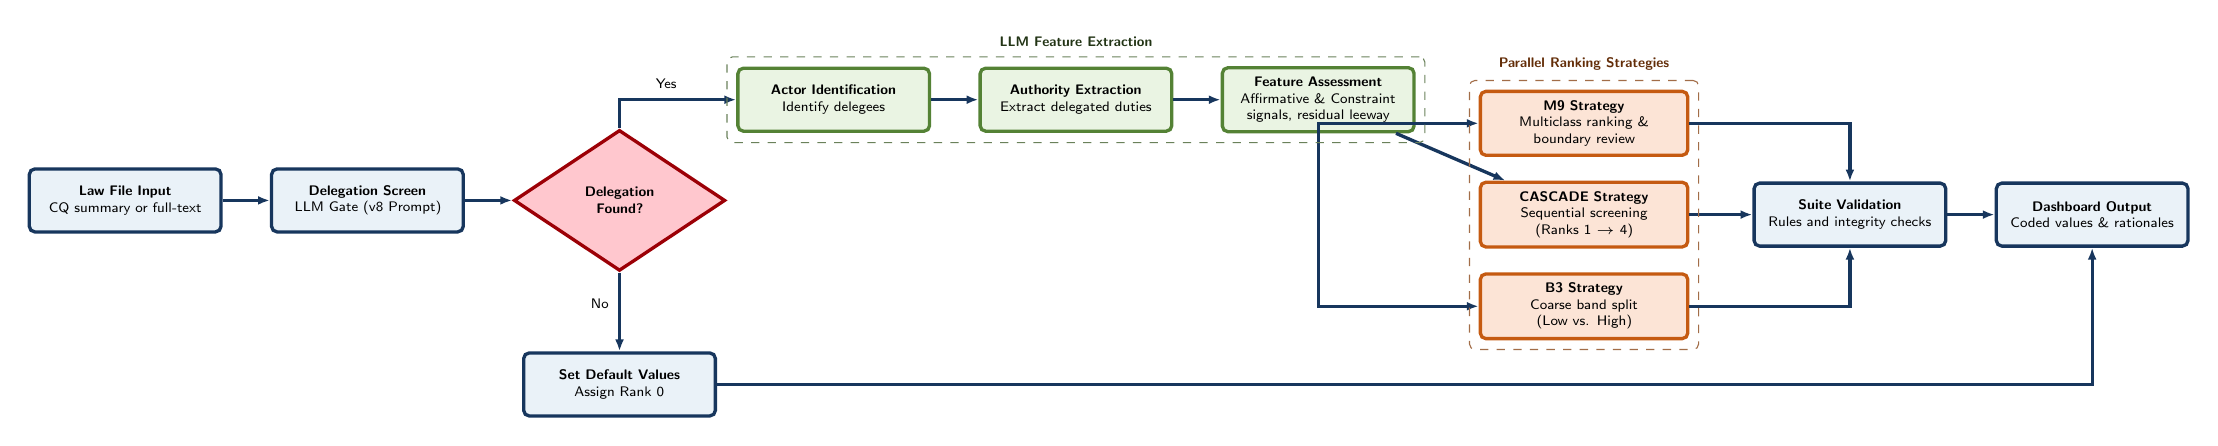
\begin{tikzpicture}[
  font=\sffamily\tiny,
  node distance=4mm and 6mm,
  box/.style={
    draw=navy,
    rounded corners=2pt,
    very thick,
    align=center,
    minimum height=8mm,
    text width=22mm,
    fill=lightblue
  },
  decision/.style={
    draw=reviewred,
    diamond,
    aspect=1.5,
    very thick,
    align=center,
    minimum height=8mm,
    text width=16mm,
    fill=reviewfill
  },
  extractor/.style={
    draw=green,
    rounded corners=2pt,
    very thick,
    align=center,
    minimum height=8mm,
    text width=22mm,
    fill=lightgreen
  },
  strategy/.style={
    draw=orange,
    rounded corners=2pt,
    very thick,
    align=center,
    minimum height=8mm,
    text width=24mm,
    fill=lightorange
  },
  arrow/.style={-{Latex[length=1.5mm]},very thick,draw=navy},
  dashedarrow/.style={-{Latex[length=1.5mm]},thick,dashed,draw=navy}
]

% 1. Input and Gate
\node[box] (input) {\textbf{Law File Input}\\CQ summary or full-text};
\node[box,right=of input] (gate) {\textbf{Delegation Screen}\\LLM Gate (v8 Prompt)};
\node[decision,right=of gate] (decision) {\textbf{Delegation\\Found?}};

% 2. No-delegation branch (bottom)
\node[box,below=10mm of decision] (nodeleg) {\textbf{Set Default Values}\\Assign Rank 0};

% 3. Extraction Phase (top)
\node[extractor,above right=4mm and 8mm of decision] (actors) {\textbf{Actor Identification}\\Identify delegees};
\node[extractor,right=of actors] (auth) {\textbf{Authority Extraction}\\Extract delegated duties};
\node[extractor,right=of auth] (signals) {\textbf{Feature Assessment}\\Affirmative \& Constraint signals, residual leeway};

% 4. Parallel Strategies
\node[strategy,below right=6mm and 8mm of signals] (cascade) {\textbf{CASCADE Strategy}\\Sequential screening\\(Ranks 1 $\rightarrow$ 4)};
\node[strategy,above=3mm of cascade] (m9) {\textbf{M9 Strategy}\\Multiclass ranking \&\\boundary review};
\node[strategy,below=3mm of cascade] (b3) {\textbf{B3 Strategy}\\Coarse band split\\(Low vs. High)};

% 5. Validation and Output
\node[box,right=8mm of cascade] (validate) {\textbf{Suite Validation}\\Rules and integrity checks};
\node[box,right=of validate] (output) {\textbf{Dashboard Output}\\Coded values \& rationales};

% Connections
\draw[arrow] (input) -- (gate);
\draw[arrow] (gate) -- (decision);
\draw[arrow] (decision) -- node[left,pos=0.4] {No} (nodeleg);
\draw[arrow] (decision) |- node[above,pos=0.7] {Yes} (actors);
\draw[arrow] (actors) -- (auth);
\draw[arrow] (auth) -- (signals);

\draw[arrow] (signals) |- (m9);
\draw[arrow] (signals) -- (cascade);
\draw[arrow] (signals) |- (b3);

\draw[arrow] (m9) -| (validate);
\draw[arrow] (cascade) -- (validate);
\draw[arrow] (b3) -| (validate);
\draw[arrow] (validate) -- (output);
\draw[arrow] (nodeleg) -| (output);

% Containers
\node[draw=green!50!gray,dashed,rounded corners=2pt,fit=(actors)(auth)(signals),label={[font=\sffamily\tiny\bfseries,text=green!40!black]above:LLM Feature Extraction}] {};
\node[draw=orange!50!gray,dashed,rounded corners=2pt,fit=(m9)(cascade)(b3),label={[font=\sffamily\tiny\bfseries,text=orange!50!black]above:Parallel Ranking Strategies}] {};

\end{tikzpicture}
}
\caption{Modular architecture of the \systemname{} workflow graph (\texttt{Version 4 - Detailed}). Upstream outputs flow into parallel CASCADE (sequential), M9 (multiclass), and B3 (coarse split) ranking strategies, followed by validation checks and final output serialization.}
\label{fig:workflow_dag}
\end{figure*}

The system evolved through repeated attempts to make the coding rule both more accurate and more interpretable. Table~\ref{tab:evolution} groups the many prompt files into four methodological phases.

\begin{table*}[t]
\centering
\caption{Development from prompt-only classification to a workflow research instrument.}
\label{tab:evolution}
\small
\begin{tabularx}{\textwidth}{@{}p{0.11\textwidth}p{0.16\textwidth}X X p{0.15\textwidth}@{}}
\toprule
\textbf{Phase} & \textbf{Representation} & \textbf{Methodological change} & \textbf{Observed motivation} & \textbf{Auditability} \\
\midrule
I & One-shot prompt & Joint binary delegation and 0--4 discretion prediction with rationale and evidence; enforce no-delegation $\Rightarrow$ rank 0. & Establish a first end-to-end coding baseline. & Final rationale, but stage errors remain entangled. \\
\addlinespace
II & Decomposed prompt & Separate label-only and rationale-bearing tasks; then separate delegation, amount/centrality, constraints, constraint categories, and rank. & Isolate output-design effects and identify where reasoning fails. & Stage text is visible, but ordering is still embedded in prompt files. \\
\addlinespace
III & Coding-sheet-aligned staged prompt & Map stages to explicit variables; tighten definitions for agency creation, appointment, external audit, sunset provisions, financial-domain scope, and omnibus laws. & Reduce false positives and align outputs with the professor's historical coding sheet. & Intermediate variables are explicit but not yet a reusable executable graph. \\
\addlinespace
IV & Versioned workflow & Convert prompts into typed nodes, upstream dependencies, conditions, deterministic assignments, validations, outputs, reusable templates, execution traces, and published snapshots. & Make the method human-editable, testable, and reproducible across documents and models. & Node-level values, rationales, timing, provenance, and branch decisions are inspectable. \\
\bottomrule
\end{tabularx}
\end{table*}

\subsection{Why a workflow rather than a larger prompt?}

The final rank depends on earlier judgments. A model should first determine whether a qualifying delegation exists, then inventory administrative actors and authority, assess the breadth and centrality of that authority, identify constraints, and only then estimate residual leeway. If no delegation exists, the workflow assigns rank 0 deterministically instead of spending another model call on an inapplicable question. If delegation exists, the rank stage receives the earlier values and rationales explicitly.

This dependency structure addresses a recurrent failure of independent-column coding: a later variable such as \texttt{discretion\_rank} cannot reliably use an earlier delegation decision unless the pipeline stores and forwards it. In the prototype, execution order is computed from the graph rather than assumed from the visual order of columns. Each node records inputs, outputs, status, timing, and, where applicable, evidence and rationale.

\subsection{Workflow primitives}
The implemented engine supports document-input, LLM, condition, deterministic set-value, validation, output, and rank-descriptor nodes. A workflow definition stores its nodes, edges, typed outputs, and metadata as a database-managed artifact (represented visually in Figure~\ref{fig:workflow_dag}). Researchers can create a workflow from a template, duplicate it, import or export its JSON representation, edit its draft, validate it, test it, and publish a numbered snapshot with a changelog and definition hash.

The distinction between \emph{workflow} and \emph{campaign} is central. A workflow defines the research instrument: concepts, prompts, stages, dependencies, branching, and outputs. A campaign or evaluation run applies a selected definition to a document collection under a specified model policy and stores the resulting dataset and traces.

\section{Human-in-the-Loop Design}

Figure~\ref{fig:hitl} presents the proposed research process. Solid arrows correspond to implemented or directly supported interactions. The dashed arrow denotes a planned governance step in which selected case-level lessons are deliberately promoted into a new workflow version; corrections do not currently retrain or silently alter the method.

\begin{figure*}[t]
\centering
\resizebox{\textwidth}{!}{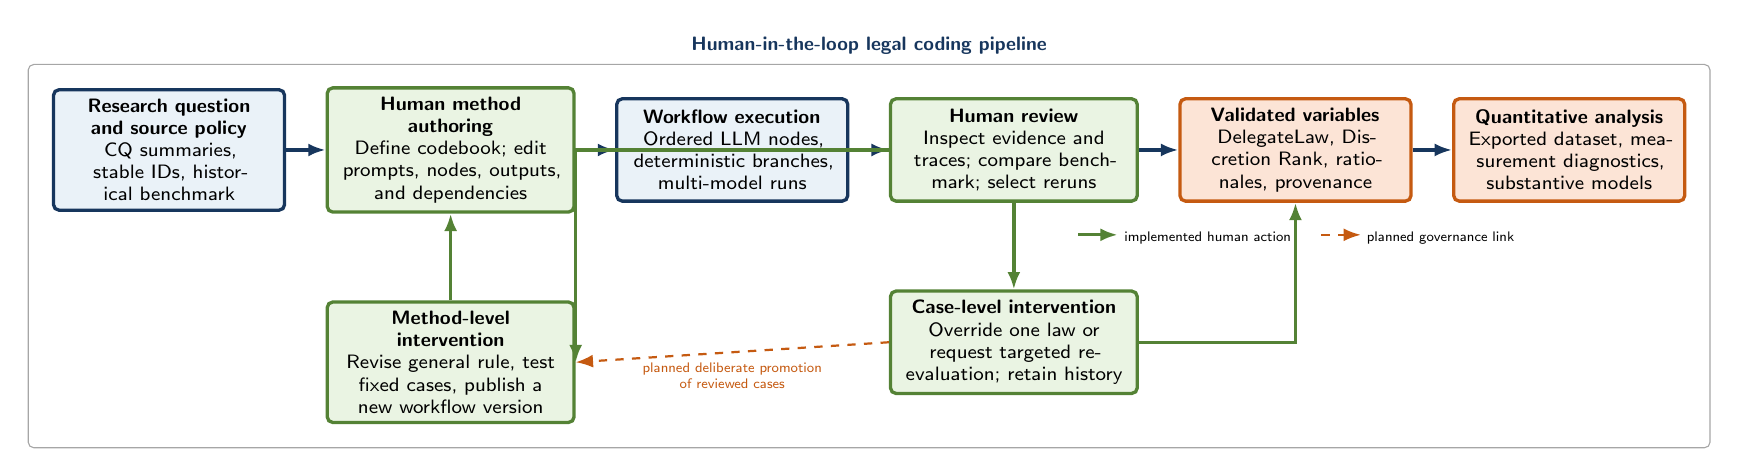
\begin{tikzpicture}[
  font=\sffamily\scriptsize,
  node distance=5mm and 5mm,
  stage/.style={
    draw=navy,
    rounded corners=2pt,
    very thick,
    align=center,
    minimum height=13mm,
    text width=27mm,
    fill=lightblue
  },
  human/.style={
    draw=green,
    rounded corners=2pt,
    very thick,
    align=center,
    minimum height=13mm,
    text width=29mm,
    fill=lightgreen
  },
  output/.style={
    draw=orange,
    rounded corners=2pt,
    very thick,
    align=center,
    minimum height=13mm,
    text width=27mm,
    fill=lightorange
  },
  arrow/.style={-{Latex[length=2.2mm]},very thick,draw=navy},
  feedback/.style={-{Latex[length=2.2mm]},very thick,draw=green},
  planned/.style={-{Latex[length=2.2mm]},thick,dashed,draw=orange}
]

\node[stage] (question) {\textbf{Research question\\and source policy}\\CQ summaries, stable IDs, historical benchmark};
\node[human,right=of question] (author) {\textbf{Human method authoring}\\Define codebook; edit prompts, nodes, outputs, and dependencies};
\node[stage,right=of author] (execute) {\textbf{Workflow execution}\\Ordered LLM nodes, deterministic branches, multi-model runs};
\node[human,right=of execute] (review) {\textbf{Human review}\\Inspect evidence and traces; compare benchmark; select reruns};
\node[output,right=of review] (variables) {\textbf{Validated variables}\\DelegateLaw, Discretion Rank, rationales, provenance};
\node[output,right=of variables] (analysis) {\textbf{Quantitative analysis}\\Exported dataset, measurement diagnostics, substantive models};

\draw[arrow] (question) -- (author);
\draw[arrow] (author) -- (execute);
\draw[arrow] (execute) -- (review);
\draw[arrow] (review) -- (variables);
\draw[arrow] (variables) -- (analysis);

\node[human,below=11mm of review] (case) {\textbf{Case-level intervention}\\Override one law or request targeted re-evaluation; retain history};
\node[human,below=11mm of author] (method) {\textbf{Method-level intervention}\\Revise general rule, test fixed cases, publish a new workflow version};

\draw[feedback] (review) -- (case);
\draw[feedback] (case.east) -| (variables.south);
\draw[feedback] (review.west) -| (method.east);
\draw[feedback] (method) -- (author);
\draw[planned] (case.west) -- node[below,align=center,text=orange,font=\sffamily\tiny]{planned deliberate promotion\\of reviewed cases} (method.east);

\node[draw=gray!70,rounded corners=2pt,fit=(question)(analysis)(method)(case),inner sep=3mm,label={[font=\sffamily\scriptsize\bfseries,text=navy]above:Human-in-the-loop legal coding pipeline}] {};

\node[below=2mm of variables,font=\sffamily\tiny,align=left] (legend) {%
\tikz\draw[feedback] (0,0)--(5mm,0); implemented human action\qquad
\tikz\draw[planned] (0,0)--(5mm,0); planned governance link};
\end{tikzpicture}
}
\caption{Human-in-the-loop legal coding pipeline. The prototype supports method-level intervention through editable workflows and case-level intervention through inspection, override, and targeted re-evaluation. A case correction changes that law's stored value; a separate, deliberate workflow revision is required to change the research instrument. Dashed elements denote planned extensions.}
\label{fig:hitl}
\end{figure*}

\subsection{Method-level intervention}

The Stage Builder exposes source-text policy, evaluation mode, calibration settings, each stage's purpose and prompt, typed output fields, and whether a field is final or retained only for audit. A live preview shows the compiled prompt. The more general graph editor exposes upstream-field selection, conditional routing, deterministic assignments, validations, and rank-specific criteria. This lets a domain expert revise the operational codebook without editing application source code.

\begin{figure*}[t]
\centering
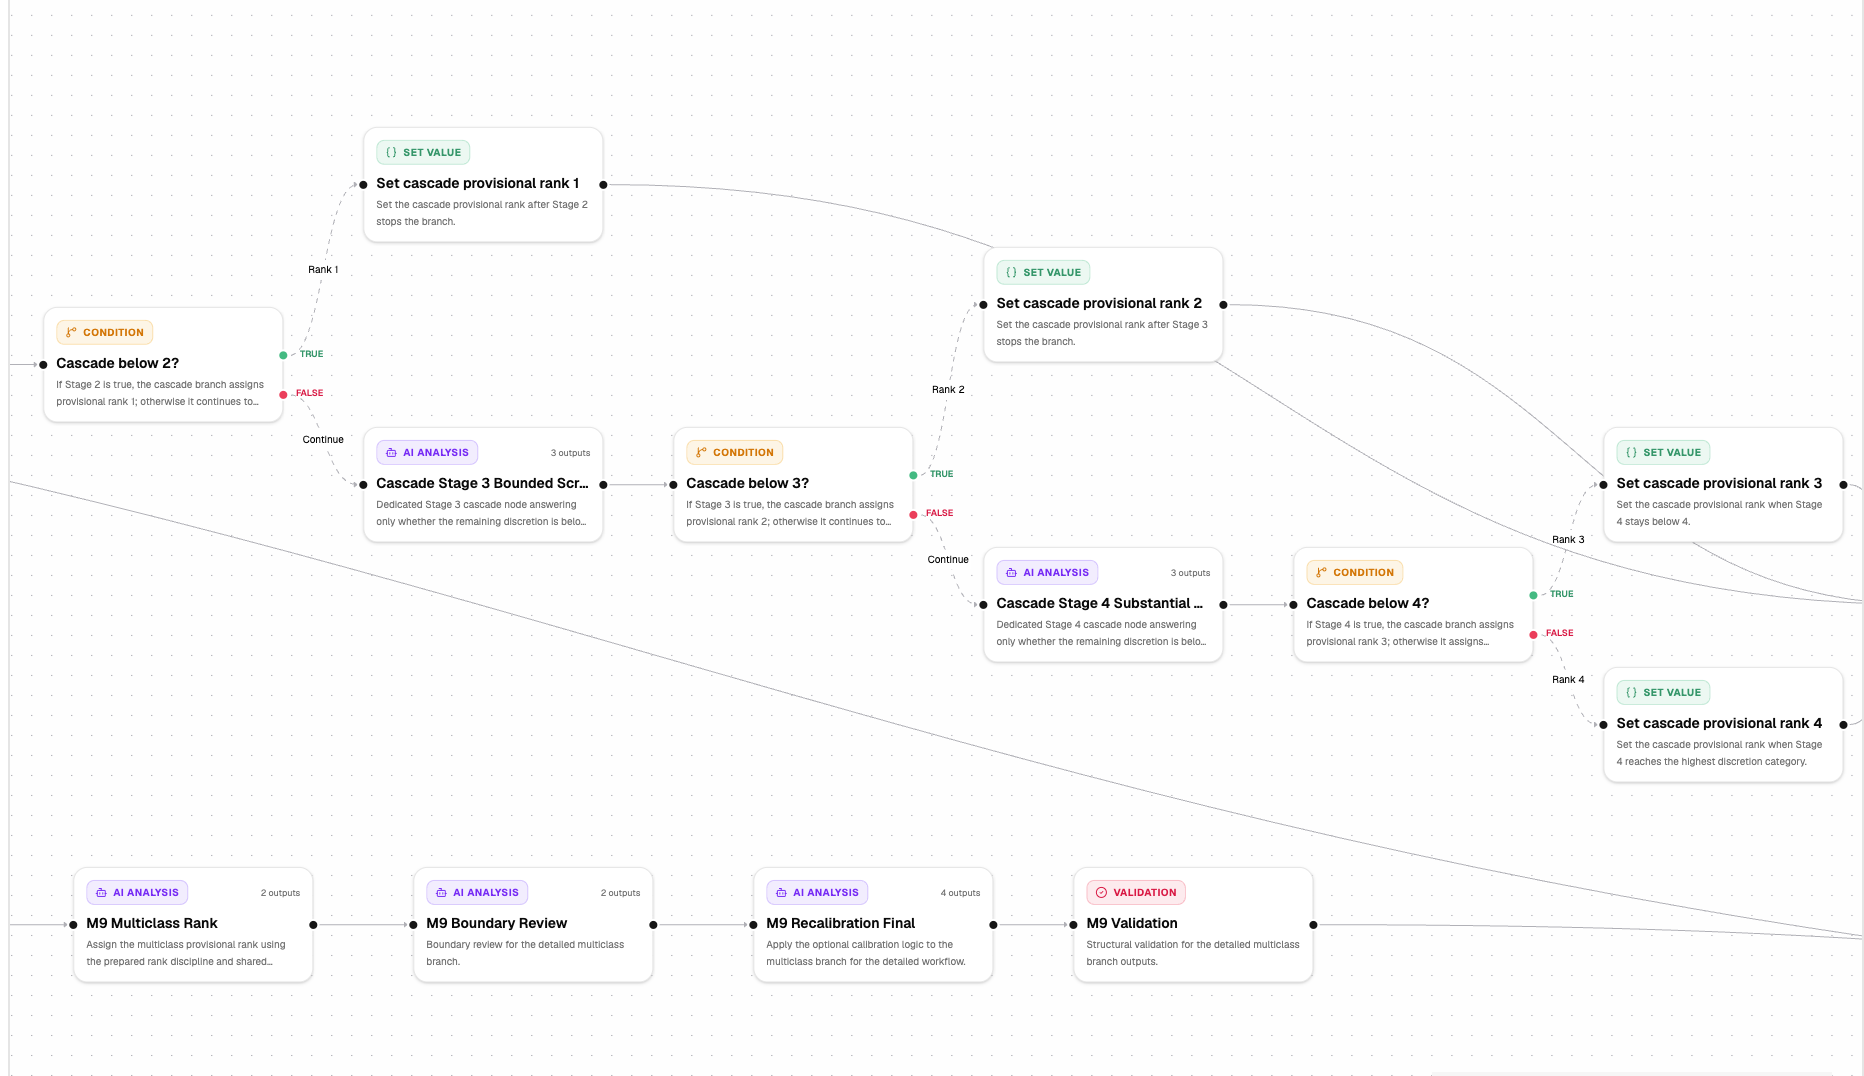
\includegraphics[width=0.96\textwidth]{figures/Workflow.png}
\caption{Product view of the workflow graph, showing how the discretion-rank task is decomposed into explicit LLM analysis nodes, condition nodes, deterministic set-value nodes, validation nodes, and connected branches. This interface exposes the coding method as an editable research instrument rather than a single hidden prompt.}
\label{fig:workflow_product}
\end{figure*}

Publishing creates an immutable numbered definition snapshot, but the current prototype does not implement a separate professor-approval request or sign-off state. Any authorized editor can publish. Similarly, the current user interface does not yet provide a complete published-version comparison and pinning workflow for all campaign types. We therefore describe publishing as a reproducibility primitive, not as a completed governance protocol.

\subsection{Case-level intervention}

For an individual coded law, a researcher can inspect the final values and the node-by-node execution trace, manually override a selected value and rationale, or request AI re-evaluation with corrective feedback. History distinguishes initial AI output, manual override, and AI re-evaluation. A manual correction is local to that law; it does not automatically change the codebook, the prompt, or other cases.

This separation is scientifically useful. Case correction protects the dataset from a known error, whereas method revision changes the coding rule and should trigger a new version and controlled rerun. The prototype therefore avoids an opaque ``learning'' process in which corrections silently alter subsequent classifications.

\subsection{Implemented boundary}

The current implementation has two authoring surfaces. Builder-backed workflows present a readable sequence of domain stages whose prompts and output metadata can be edited, but their compiled graph is currently read-only and the stage sequence is determined by the selected mode. The generic graph editor permits lower-level node and edge authoring. Validation nodes currently report diagnostic flags but do not halt execution. Role-specific professor/research-assistant/student permissions, formal approval gates, automatic promotion of case corrections, and a hard-case review queue are future extensions.

\section{Experimental Design}

\subsection{Controlled prompt comparison}

The professor-authored testing protocol fixes a development set, holds source documents constant, records prompt and model versions, preserves law identifiers, and compares each output with the manual benchmark. After each revision, the same laws are rerun and disagreements are reviewed law by law. The protocol explicitly distinguishes recurring errors from isolated mistakes.

The recorded error taxonomy includes: treating any delegation as high discretion; treating minor technical delegation as central; missing constraints; treating rulemaking authority as unconstrained when standards or procedures exist; inventing authority not found in the supplied text; relying on full-text evidence absent from the summary; producing a final rank inconsistent with earlier stages; and confusing delegation with discretion.

The canonical 15-law development set is composed of the 13 delegation-positive summaries available in the summary folder, supplemented by two delegation-negative cases from the broader corpus (PL96-3 and PL92-165) to support class-balanced evaluation.

\subsection{Model and workflow comparison}

The evaluation dashboard can lock one workflow definition, apply it to the same files across multiple selected models, retain model-keyed values and traces, and report per-variable matches, rank error, token use, cost, timing, and failures. This design separates the coding strategy from the model used to execute it.

The campaign evaluation interface can summarize model-level costs, token use, per-strategy benchmark agreement, mapped cells, and variable-level matches. Figure~\ref{fig:ai_benchmark} shows a compact product view of this comparison for two selected models.

\begin{figure}[t]
\centering
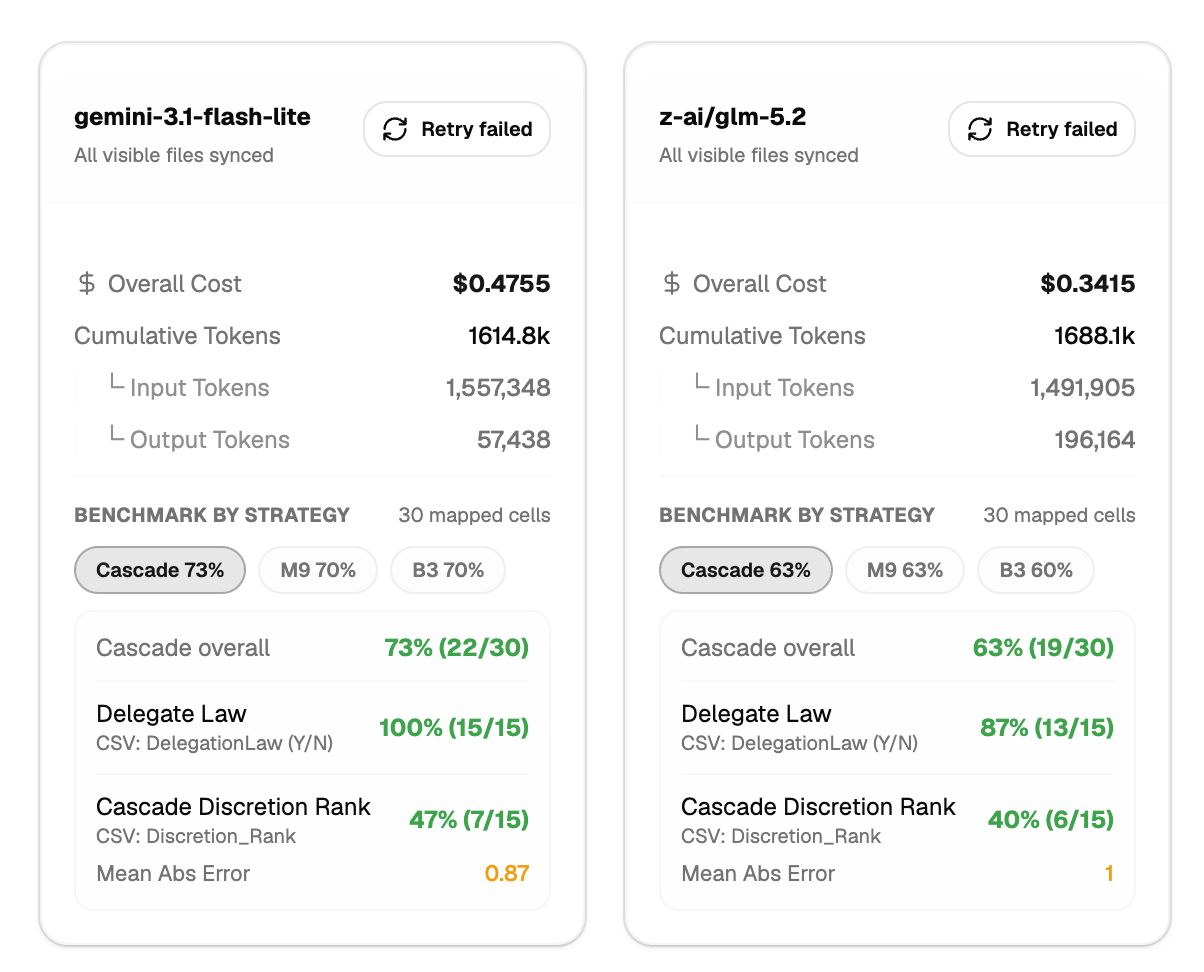
\includegraphics[width=0.95\columnwidth]{figures/AI_Benchmark.png}
\caption{Benchmark-comparison interface showing model-level cost, token counts, strategy-level agreement, and variable-level matches for selected models.}
\label{fig:ai_benchmark}
\end{figure}

\subsection{Metrics}

For the binary task, we report overall accuracy, positive-class recall, negative-class recall, and balanced accuracy. If the historical positive class is delegation, then
\[
\mathrm{BalancedAccuracy}
=\tfrac{1}{2}\left(
\frac{\mathrm{TP}}{\mathrm{TP}+\mathrm{FN}}
+
\frac{\mathrm{TN}}{\mathrm{TN}+\mathrm{FP}}
\right).
\]
For the ordinal discretion task, the evaluation interface supports exact accuracy, accuracy within one rank, mean absolute error (MAE), and a 0--4 confusion matrix. These measures distinguish an adjacent-rank disagreement from a substantively larger error.

\section{Preliminary Findings}

\subsection{Binary delegation}

Table~\ref{tab:binary} reconstructs metrics from persisted local dashboard rows. The benchmark is severely imbalanced: 161 positive cases and only eight negative cases. An always-positive classifier would obtain 95.27\% raw accuracy while failing every negative case. Raw accuracy is therefore not an adequate measure of whether prompt refinement improves the underlying coding rule.

\begin{table*}[t]
\centering
\caption{Preliminary binary delegation results reconstructed from persisted dashboard rows. Positive denotes the historical delegation-positive class.}
\label{tab:binary}
\small
\begin{tabular}{@{}lrrrrrrrrr@{}}
\toprule
\textbf{Strategy} & \textbf{N} & \textbf{TP} & \textbf{FN} & \textbf{TN} & \textbf{FP} & \textbf{Accuracy} & \textbf{Pos. recall} & \textbf{Neg. recall} & \textbf{Balanced acc.} \\
\midrule
Prompt v7, Stage 1 v4 & 169 & 156 & 5 & 4 & 4 & 94.67\% & 96.89\% & 50.00\% & 73.45\% \\
Prompt v8 & 169 & 148 & 13 & 7 & 1 & 91.72\% & 91.93\% & 87.50\% & 89.71\% \\
\bottomrule
\end{tabular}
\vspace{0.3em}

\raggedright\footnotesize Model: \texttt{gemini-3.1-flash-lite-preview}. Runs were executed on June 20, 2026. The v8 subsets (8 negative and 161 positive documents) are combined here as a single evaluation series.
\end{table*}

The looser v7 strategy yields the better raw accuracy because it preserves positive-class recall. The conservative v8 strategy makes more false-negative errors, but it detects seven of the eight rare negative cases and produces a much higher balanced accuracy. The substantive result is therefore a trade-off, not a monotonic claim that one prompt is ``more accurate.'' If the research priority is recovering rare non-delegation cases for expert review, v8 is the stronger baseline. If the priority is maximizing delegation recall, v7 is stronger.

\subsection{A calibration failure}

The law PL83-577 illustrates why source discipline and intermediate evidence matter. The historical CSV codes it as non-delegation with rank 0. An exploratory staged full-text run instead identified Securities and Exchange Commission rulemaking and exemption authority and returned delegation with rank 3. This disagreement could reflect an overbroad coding rule, a source-universe difference, or a mismatch between historical summary coding and full statutory detail. A final label alone cannot distinguish these explanations; a trace that records actor, authority, source evidence, and stage decisions can.

\subsection{Discretion rank and model comparison}

Early 15-law experiments provide exploratory ordinal results (Table~\ref{tab:rank}). Exact agreement remained modest, reaching 40\% in the strongest checked runs, while 73.3\% of predictions were within one rank across all four strategies. These small-sample results motivated clearer separation of delegation screening, constraint extraction, and final ranking. They should not be treated as a held-out estimate of final workflow performance.

\begin{table}[t]
\centering
\caption{Exploratory Discretion Rank results on 15 laws. All runs used \texttt{gemini-3.1-flash-lite-preview}.}
\label{tab:rank}
\small
\begin{tabular}{@{}lrrr@{}}
\toprule
\textbf{Dashboard strategy} & \textbf{Exact} & \textbf{Within 1} & \textbf{MAE} \\
\midrule
Prompt v3   & 26.7\% & 73.3\% & 1.067 \\
Prompt v3.4 & 40.0\% & 73.3\% & 0.933 \\
Prompt v3.5 & 40.0\% & 73.3\% & 0.933 \\
Prompt v3.6 & 33.3\% & 73.3\% & 1.000 \\
\bottomrule
\end{tabular}
\vspace{0.25em}

\raggedright\footnotesize Metrics were reconstructed from persisted dashboard rows matched to the ground-truth CSV by public-law number. Campaigns v3.4, v3.5, and v3.6 share the identical prompt text (Prompt Version 7.2); variance in metrics is due to LLM nondeterminism.
\end{table}

The production interface also supports multi-model comparisons. The cross-model evaluation results on the 15-law development set are summarized in Table~\ref{tab:multimodel}. Across the six models, CASCADE generally provides the strongest exact-accuracy results, while M9 often improves within-one-rank accuracy and mean absolute error. B3 generally performs worse on this development set, but the pattern should be interpreted cautiously because the evaluation sample is small. The strongest exact-accuracy result is gemini-3.5-flash with CASCADE (50.0\%), while the lowest MAE in Table~\ref{tab:multimodel} is gemini-3.1-flash-lite with M9 (0.800).

\begin{table*}[t]
\centering
\caption{Cross-model evaluation results on the 15-law development set for CASCADE, M9, and B3 ranking strategies.}
\label{tab:multimodel}
\small
\begin{tabular}{@{}llcccc@{}}
\toprule
\textbf{Model} & \textbf{Strategy} & \textbf{Exact Accuracy} & \textbf{Within 1 Rank} & \textbf{MAE} & \textbf{N} \\
\midrule
\multirow{3}{*}{gemini-3.5-flash}
  & CASCADE & 50.0\% & 57.1\% & 0.929 & 14 \\
  & M9      & 21.4\% & 71.4\% & 1.071 & 14 \\
  & B3      & 28.6\% & 64.3\% & 1.143 & 14 \\
\midrule
\multirow{3}{*}{gemini-3.1-flash-lite}
  & CASCADE & 46.7\% & 73.3\% & 0.867 & 15 \\
  & M9      & 40.0\% & 80.0\% & 0.800 & 15 \\
  & B3      & 40.0\% & 60.0\% & 1.067 & 15 \\
\midrule
\multirow{3}{*}{qwen/qwen3-235b-a22b-2507}
  & CASCADE & 46.7\% & 60.0\% & 1.133 & 15 \\
  & M9      & 26.7\% & 73.3\% & 1.133 & 15 \\
  & B3      & 26.7\% & 46.7\% & 1.533 & 15 \\
\midrule
\multirow{3}{*}{z-ai/glm-5.2}
  & CASCADE & 40.0\% & 73.3\% & 1.000 & 15 \\
  & M9      & 40.0\% & 73.3\% & 1.000 & 15 \\
  & B3      & 33.3\% & 60.0\% & 1.133 & 15 \\
\midrule
\multirow{3}{*}{deepseek-v4-flash}
  & CASCADE & 40.0\% & 73.3\% & 0.933 & 15 \\
  & M9      & 26.7\% & 80.0\% & 1.067 & 15 \\
  & B3      & 26.7\% & 40.0\% & 1.667 & 15 \\
\midrule
\multirow{3}{*}{nousresearch/hermes-3-llama-3.1-405b}
  & CASCADE & 33.3\% & 53.3\% & 1.333 & 15 \\
  & M9      & 33.3\% & 60.0\% & 1.333 & 15 \\
  & B3      & 26.7\% & 60.0\% & 1.333 & 15 \\
\bottomrule
\end{tabular}
\end{table*}

\section{Discussion}

\subsection{The workflow as a research instrument}

The main contribution of the prototype is methodological rather than a claim of universally superior classification. The workflow externalizes decisions that were previously buried inside prompt prose: which source text is admissible, which stages must precede others, which intermediate variables are retained, when deterministic rules apply, and what information the final rank is allowed to use. The resulting artifact can be inspected, duplicated, versioned, tested, and rerun.

This design is aligned with a quantitative social-science perspective. The goal is not merely to produce plausible legal interpretations. It is to operationalize a concept consistently, compare predictions with a coded benchmark, diagnose systematic disagreements, and preserve enough provenance for another researcher to reproduce the coding process. In that sense, the workflow plays a role analogous to a versioned coding protocol or measurement instrument.

\subsection{What the human contributes}

The human remains responsible for defining constructs, choosing the source universe, approving the codebook in the substantive sense, interpreting benchmark disagreements, correcting known errors, and deciding whether a case-level lesson warrants a method-level revision. The LLM contributes scalable extraction, structured intermediate judgments, and candidate classifications. The system contributes orchestration, provenance, comparison, and versioning.

The two human loops should not be conflated. A local override is appropriate when a researcher knows that one case is wrong. A workflow revision is appropriate when the error reveals a general rule. The latter should create a new version and be evaluated on a controlled set before adoption.

\subsection{Limitations}

Several limitations bound the current evidence. First, the binary benchmark is extremely imbalanced, and prompt development on the same cases risks overfitting. Second, the benchmark is based on summaries; conclusions do not automatically transfer to full statutes. Third, no verified intercoder-reliability information is currently available for the historical labels. Fourth, a single formal run per strategy does not establish statistical stability, even if spot reruns return identical outputs. Fifth, ordinal ranks can propagate errors from earlier stages. Sixth, the current study concerns one policy domain and has no external-dataset validation. Seventh, model and provider versions can drift. Finally, some audit and governance capabilities remain incomplete: validation is diagnostic, actor-attributed override logs are limited, and workflow-version approval and pinning are not yet uniform across the product.

\subsection{Novelty claim}

Related systems separately study LLM annotation, active review, weak supervision, prompt chaining, and visual workflow authoring \citep{cormack2014evaluation,ratner2017snorkel,wu2022aichains,wu2022promptchainer}. Our cautious claim is that \systemname{} offers a potentially distinctive integration for expert-guided legal-institutional coding: a domain codebook represented as an editable dependency graph, deterministic and generative stages in one instrument, trace-linked benchmark comparison, and both method-level and case-level human intervention. A broader product comparison is still required before claiming industry uniqueness.

\section{Replication Workflow}

The current prototype can be replicated through the following research-facing sequence:

\begin{enumerate}
  \item \textbf{Prepare the corpus.} Upload CQ summaries or corresponding major-provisions text and retain stable law identifiers. Keep full statutes in a separately labeled exploratory collection.
  \item \textbf{Create the instrument.} Duplicate the delegation-and-discretion workflow template. Review every stage's purpose, prompt, required inputs, typed outputs, and final/internal visibility.
  \item \textbf{Validate and test.} Run representative positive, negative, and boundary cases. Inspect graph validation, final outputs, and node-level traces.
  \item \textbf{Freeze a version.} Save a changelog and publish a numbered workflow snapshot before a benchmark run. Linking a campaign copies the workflow's draft definition and revision directly to the dashboard, preventing subsequent edits from silently affecting active runs.
  \item \textbf{Run a controlled evaluation.} Apply the same workflow and source set across selected models or strategies. Record model identifiers, settings, timestamps, failures, token use, and cost.
  \item \textbf{Compare with ground truth.} Map benchmark columns, calculate binary class-specific metrics and ordinal rank metrics, and inspect every mismatch.
  \item \textbf{Intervene explicitly.} Correct a case locally when appropriate. If the disagreement reveals a general rule, revise the workflow separately, publish a new version, and rerun the fixed development set.
  \item \textbf{Export the dataset.} Preserve final variables alongside the workflow version, model, source universe, and audit history needed for downstream quantitative analysis.
\end{enumerate}

\section{Future Work}

Immediate empirical work should reconcile the benchmark artifacts, export the live multi-model results, evaluate discretion-rank performance, and repeat runs to characterize model variability. Methodological work should add a held-out evaluation set and, if feasible, independent recoding to estimate intercoder reliability.

Product work should add role-specific governance, workflow-version comparison and pinning, model-aware manual correction in the evaluation dashboard, editable validation rules, and a deliberate mechanism for promoting reviewed cases into a new calibration set or workflow version. External validity should be tested on an additional policy dataset before making claims beyond financial regulation.

\section{Conclusion}

This project began as an effort to improve prompts for classifying legal delegation and discretion. Its more consequential development was the recognition that prompt wording alone cannot provide the transparency, dependency management, and reproducibility required for a research coding method. The resulting prototype turns the codebook into an explicit workflow and places human judgment at two visible points: designing the method and correcting cases. Preliminary evidence shows why this structure is necessary: prompt revisions change class-specific trade-offs that raw accuracy can conceal. The next step is not to remove the human from the loop, but to make expert intervention systematic, auditable, and empirically evaluable.

\balance
\bibliographystyle{plainnat}
\bibliography{references}

\end{document}
